%# -*- coding: utf-8-unix -*-
%%==================================================
%% thesis.tex
%%==================================================

% 双面打印
\documentclass[doctor, openright, twoside]{sjtuthesis}
% \documentclass[bachelor, openany, oneside, submit]{sjtuthesis}
% \documentclass[master, review]{sjtuthesis}
% \documentclass[%
%   bachelor|master|doctor,	% 必选项
%   fontset=fandol|windows|mac|ubuntu|adobe|founder, % 字体选项
%   oneside|twoside,		% 单面打印,双面打印(奇偶页交换页边距,默认)
%   openany|openright, 		% 可以在奇数或者偶数页开新章|只在奇数页开新章(默认)
%   english,			% 启用英文模版
%   review,	 		% 盲审论文,隐去作者姓名、学号、导师姓名、致谢、发表论文和参与的项目
%   submit			% 定稿提交的论文,插入签名扫描版的原创性声明、授权声明 
% ]

% 逐个导入参考文献数据库
\addbibresource{bib/thesis.bib}
% \addbibresource{bib/chap2.bib}

\begin{document}

%% 无编号内容:中英文论文封面、授权页
%# -*- coding: utf-8-unix -*-
\title{上海交通大学学位论文 \LaTeX 模板示例文档}
\author{某\quad{}某}
\advisor{某某教授}
% \coadvisor{某某教授}
\defenddate{2014年12月17日}
\school{上海交通大学}
\institute{某某系}
\studentnumber{0010900990}
\major{某某专业}

\englishtitle{A Sample Document for \LaTeX-basedd SJTU Thesis Template}
\englishauthor{\textsc{Mo Mo}}
\englishadvisor{Prof. \textsc{Mou Mou}}
% \englishcoadvisor{Prof. \textsc{Uom Uom}}
\englishschool{Shanghai Jiao Tong University}
\englishinstitute{\textsc{Depart of XXX, School of XXX} \\
  \textsc{Shanghai Jiao Tong University} \\
  \textsc{Shanghai, P.R.China}}
\englishmajor{A Very Important Major}
\englishdate{Dec. 17th, 2014}


\maketitle

\makeatletter
\ifsjtu@submit\relax
	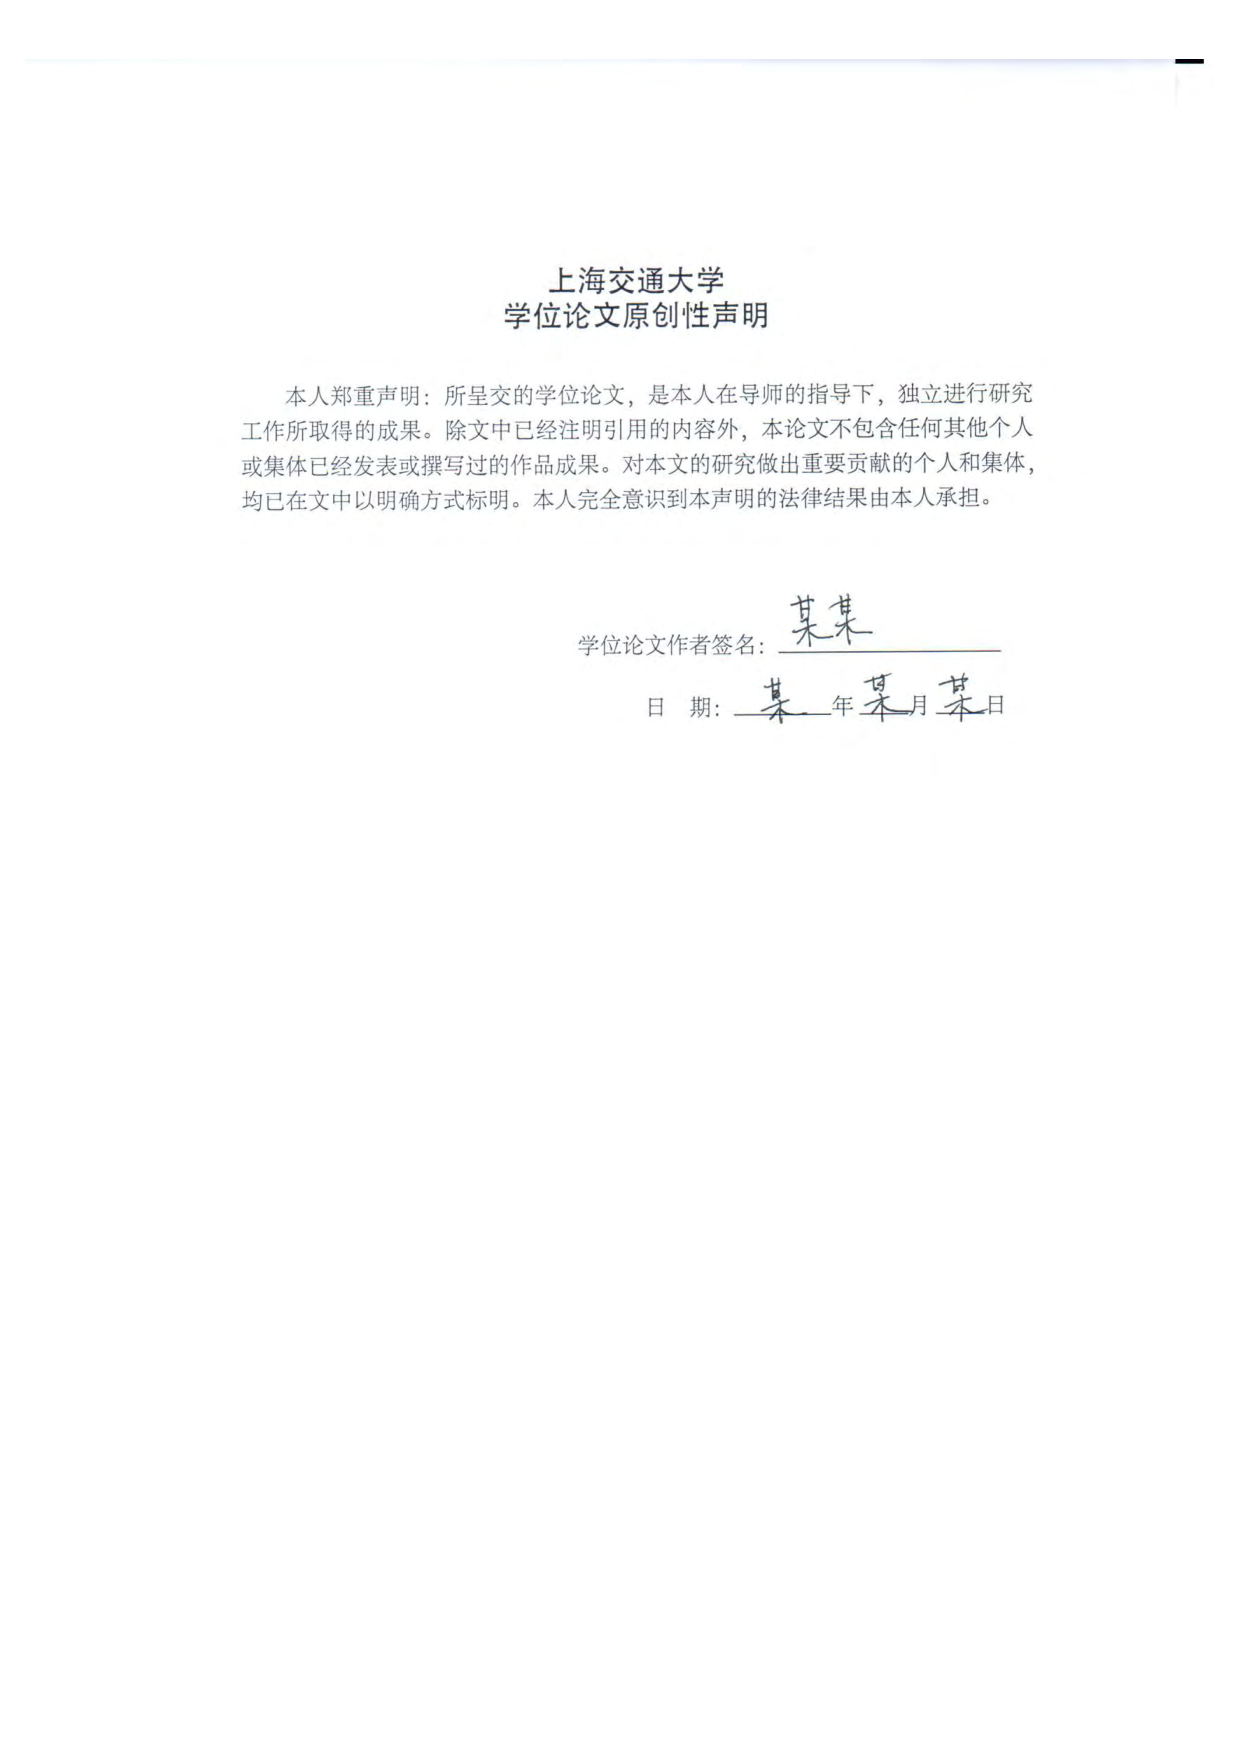
\includepdf{pdf/original.pdf}
	\cleardoublepage
	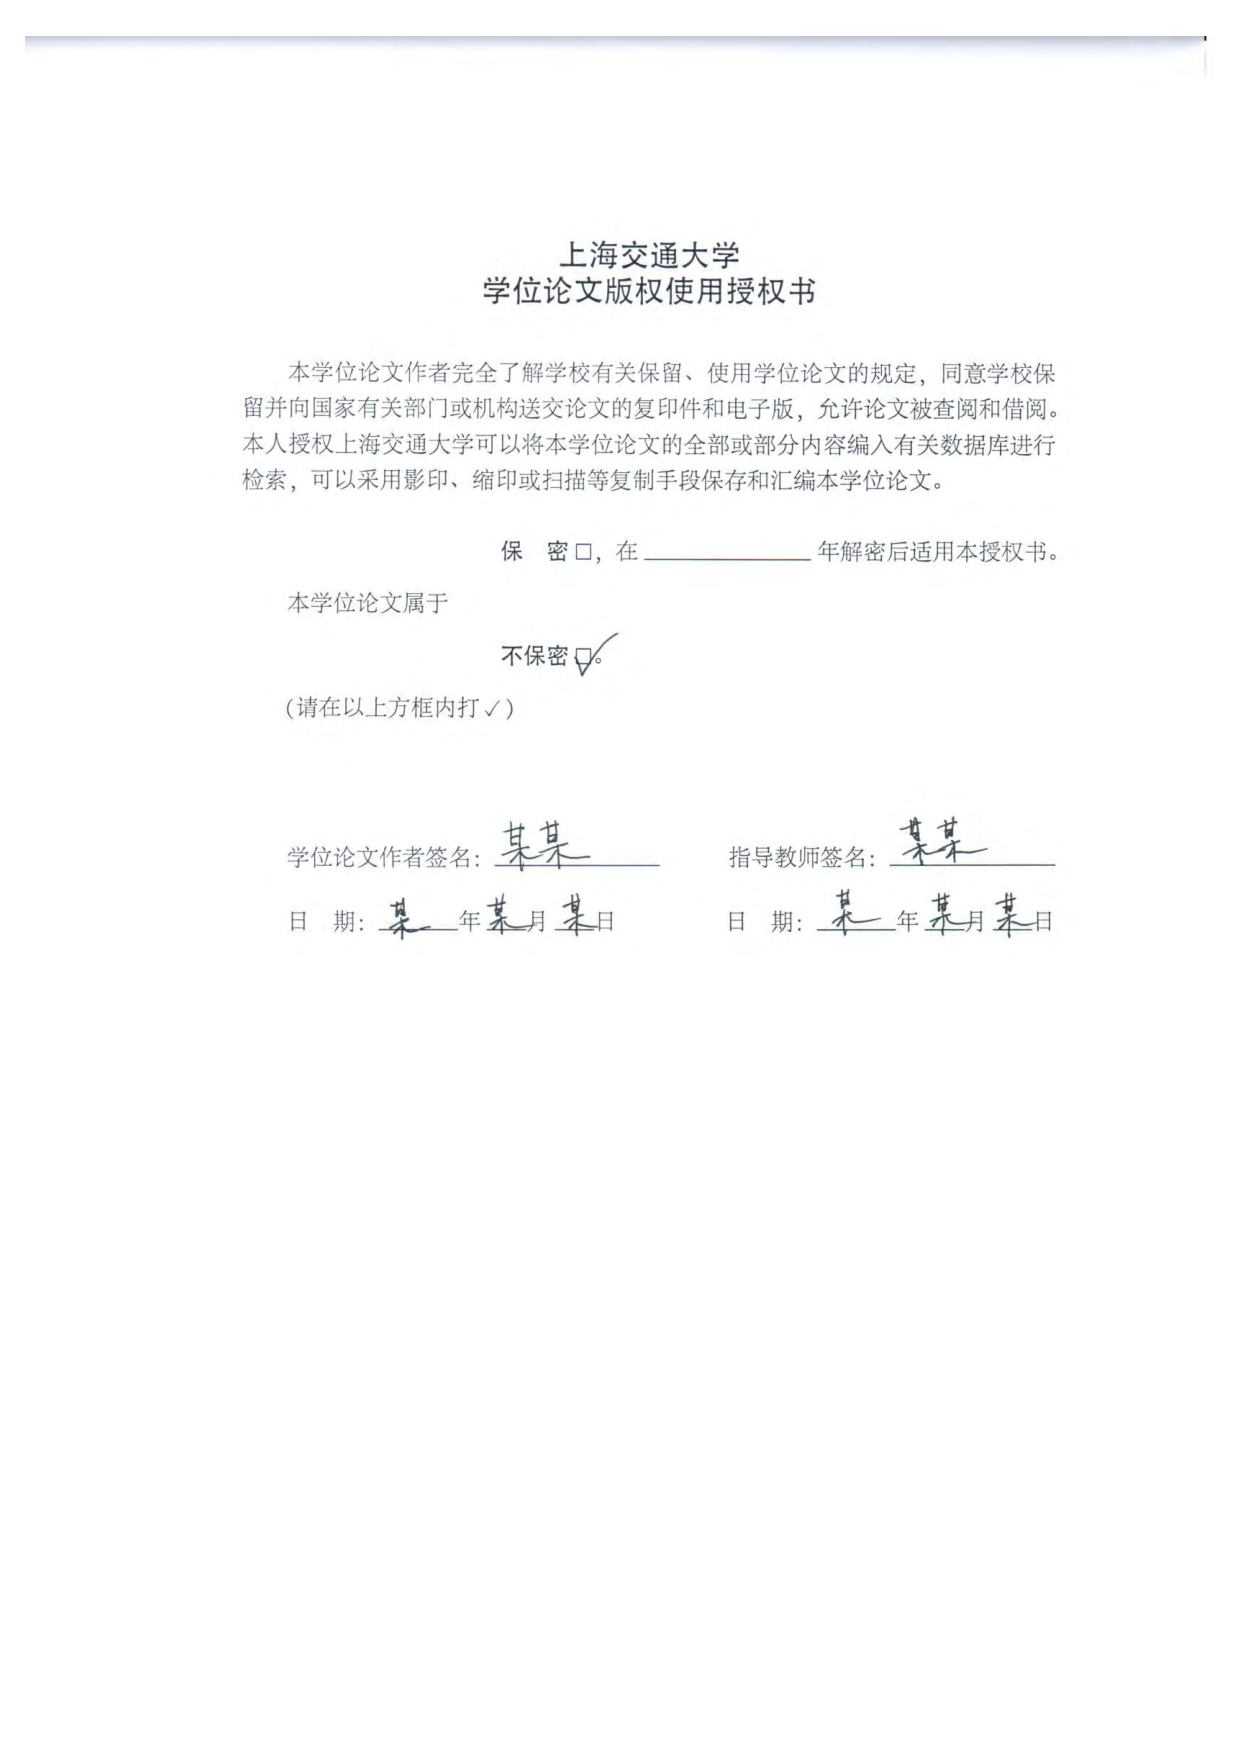
\includepdf{pdf/authorization.pdf}
	\cleardoublepage
\else
\ifsjtu@review\relax
% exclude the original claim and authorization
\else
	\makeDeclareOriginal
	\makeDeclareAuthorization
\fi
\fi
\makeatother


\frontmatter 	% 使用罗马数字对前言编号

%% 摘要
\pagestyle{main}
% Abstract
\clearpage
\thispagestyle{plain}
\phantomsection
\addcontentsline{toc}{chapter}{Abstract}

\centerline{\zihao{3}\bfseries Abstract}

\linespread{1.4}\zihao{-4}
\bigskip

This thesis explores the relationship between focus structure and pronoun resolution among non-native speakers of English and French. Firstly we reviewed the existing literature on the mechanism of focus effect and pronoun resolution. Then through a self-paced reading test, we find that focus, in the form of cleft structure does not necessarily increase the salience of a informational unit, thus may not in some cases make it a preferred antecedent for pronoun resolution. This result is line with previous researches on this topic. In our experiment, We also find that focused subject in French and focused object in English are processed faster, but focused subjects in both languages leads to longer response time of anaphora. Furthermore, our research also shows that the congruence between anaphora and focus does not make the latter more accessible. In this regard, we argue that the problem of whether there is subject or object preference in English and French is more complicated than the results of current studies.

\bigskip
\noindent\textbf{\zihao{4} Keywords:} 
focus effect, pronoun resolution, self-paced reading, English, French



%% 目录、插图目录、表格目录
\tableofcontents
\listoffigures
\addcontentsline{toc}{chapter}{\listfigurename} %将插图目录加入全文目录
\listoftables
\addcontentsline{toc}{chapter}{\listtablename}  %将表格目录加入全文目录
\listofalgorithms
\addcontentsline{toc}{chapter}{\listalgorithmname} %将算法目录加入全文目录

%# -*- coding: utf-8-unix -*-
\begin{nomenclaturename}
\label{chap:symb}

\begin{longtable}{rl}
$\epsilon$     & 介电常数 \\
 $\mu$ 		& 磁导率 \\
 $\epsilon$     & 介电常数 \\
 $\mu$ 		& 磁导率 \\
 $\epsilon$     & 介电常数 \\
 $\mu$ 		& 磁导率 \\
 $\epsilon$ 	& 介电常数 \\
 $\mu$ 		& 磁导率 \\
 $\epsilon$     & 介电常数 \\
 $\mu$ 		& 磁导率 \\
 $\epsilon$     & 介电常数 \\
 $\mu$ 		& 磁导率 \\
 $\epsilon$     & 介电常数 \\
 $\mu$ 		& 磁导率 \\
 $\epsilon$ 	& 介电常数 \\
 $\mu$ 		& 磁导率 \\
 $\epsilon$     & 介电常数 \\
 $\mu$ 		& 磁导率 \\
 $\epsilon$     & 介电常数 \\
 $\mu$ 		& 磁导率 \\
 $\epsilon$     & 介电常数 \\
 $\mu$ 		& 磁导率 \\
 $\epsilon$ 	& 介电常数 \\
 $\mu$ 		& 磁导率 \\
 $\epsilon$     & 介电常数 \\
 $\mu$ 		& 磁导率 \\
 $\epsilon$     & 介电常数 \\
 $\mu$ 		& 磁导率 \\
 $\epsilon$     & 介电常数 \\
 $\mu$ 		& 磁导率 \\
 $\epsilon$ 	& 介电常数 \\
 $\mu$ 		& 磁导率 \\
 $\epsilon$     & 介电常数 \\
 $\mu$ 		& 磁导率 \\
 $\epsilon$     & 介电常数 \\
 $\mu$ 		& 磁导率 \\
 $\epsilon$     & 介电常数 \\
 $\mu$ 		& 磁导率 \\
 $\epsilon$ 	& 介电常数 \\
 $\mu$ 		& 磁导率 \\
 $\epsilon$     & 介电常数 \\
 $\mu$ 		& 磁导率 \\
 $\epsilon$     & 介电常数 \\
 $\mu$ 		& 磁导率 \\
 $\epsilon$     & 介电常数 \\
 $\mu$ 		& 磁导率 \\
 $\epsilon$ 	& 介电常数 \\
 $\mu$ 		& 磁导率 \\
 $\epsilon$     & 介电常数 \\
 $\mu$ 		& 磁导率 \\
 $\epsilon$     & 介电常数 \\
 $\mu$ 		& 磁导率 \\
 $\epsilon$     & 介电常数 \\
 $\mu$ 		& 磁导率 \\
\end{longtable}

\end{nomenclaturename}
 % 主要符号、缩略词对照表

\mainmatter	% 使用阿拉伯数字对正文编号

%% 正文内容
\pagestyle{main}
%# -*- coding: utf-8-unix -*-
%%==================================================
%% chapter01.tex for SJTU Master Thesis
%%==================================================

%\bibliographystyle{sjtu2}%[此处用于每章都生产参考文献]
\chapter{这是什么}
\label{chap:intro}

这是上海交通大学(非官方)学位论文 \LaTeX 模板,当前版本是 \version 。

最早的一版学位模板是一位热心的物理系同学制作的。
那份模板参考了自动化所学位论文模板,使用了CASthesis.cls文档类,中文字符处理则采用当时最为流行的 \CJKLaTeX 方案。
我根据交大研究生院对学位论文的要求
\footnote{\url{http://www.gs.sjtu.edu.cn/policy/fileShow.ahtml?id=130}}
,结合少量个人审美喜好,完成了一份基本可用的交大 \LaTeX 学位论文模板。
但是,搭建一个 \CJKLaTeX 环境并不简单,单单在Linux下配置环境和添加中文字体,就足够让新手打退堂鼓。
在William Wang的建议下,我开始着手把模板向 \XeTeX 引擎移植。
他完成了最初的移植,多亏了他出色的工作,后续的改善工作也得以顺利进行。

随着我对 \LaTeX 系统认知增加,我又断断续续做了一些完善模板的工作,在原有硕士学位论文模板的基础上完成了交大学士和博士学位论文模板。

现在,交大学位论文模板SJTUTHesis代码在github
\footnote{\url{https://github.com/sjtug/SJTUThesis}}
上维护。
你可以\href{https://github.com/sjtug/SJTUThesis/issues}{在github上开issue}
、或者在\href{https://bbs.sjtu.edu.cn/bbsdoc?board=TeX_LaTeX}{水源LaTeX版}发帖来反映遇到的问题。

\section{使用模板}

\subsection{准备工作}
\label{sec:requirements}

要使用这个模板撰写学位论文,需要在\emph{TeX系统}、\emph{TeX技能}上有所准备。

\begin{itemize}[noitemsep,topsep=0pt,parsep=0pt,partopsep=0pt]
	\item {\TeX}系统:所使用的{\TeX}系统要支持 \XeTeX 引擎,且带有ctex 2.x宏包,以2015年的\emph{完整}TeXLive、MacTeX发行版为佳。
	\item TeX技能:尽管提供了对模板的必要说明,但这不是一份“ \LaTeX 入门文档”。在使用前请先通读其他入门文档。
	\item 针对Windows用户的额外需求:学位论文模本分别使用git和GNUMake进行版本控制和构建,建议从Cygwin\footnote{\url{http://cygwin.com}}安装这两个工具。
\end{itemize}

\subsection{模板选项}
\label{sec:thesisoption}

sjtuthesis提供了一些常用选项,在thesis.tex在导入sjtuthesis模板类时,可以组合使用。
这些选项包括:

\begin{itemize}[noitemsep,topsep=0pt,parsep=0pt,partopsep=0pt]
	\item 学位类型:bachelor(学位)、master(硕士)、doctor(博士),是必选项。
	\item 中文字体:fandol(Fandol 开源字体)、windows(Windows 系统下的中文字体)、mac(macOS 系统下的华文字体)、ubuntu(Ubuntu 系统下的文泉驿和文鼎字体)、adobe(Adobe 公司的中文字体)、founder(方正公司的中文字体),默认根据操作系统自动配置。
	\item 英文模版:使用english选项启用英文模版。
	\item 盲审选项:使用review选项后,论文作者、学号、导师姓名、致谢、发表论文和参与项目将被隐去。
\end{itemize}

\subsection{编译模板}
\label{sec:process}

模板默认使用GNUMake构建,GNUMake将调用latemk工具自动完成模板多轮编译:

\begin{lstlisting}[basicstyle=\small\ttfamily, caption={编译模板}, numbers=none]
make clean thesis.pdf
\end{lstlisting}

若需要生成包含“原创性声明扫描件”的学位论文文档,请将扫描件保存为statement.pdf,然后调用make生成submit.pdf。

\begin{lstlisting}[basicstyle=\small\ttfamily, caption={生成用于提交的学位论文}, numbers=none]
make clean submit.pdf
\end{lstlisting}

编译失败时,可以尝试手动逐次编译,定位故障。

\begin{lstlisting}[basicstyle=\small\ttfamily, caption={手动逐次编译}, numbers=none]
xelatex -no-pdf thesis
biber --debug thesis
xelatex thesis
xelatex thesis
\end{lstlisting}

\subsection{模板文件布局}
\label{sec:layout}

\begin{lstlisting}[basicstyle=\small\ttfamily,caption={模板文件布局},label=layout,float,numbers=none]
├── LICENSE
├── Makefile
├── README.md
├── bib
│   ├── chap1.bib
│   └── chap2.bib
├── bst
│   └── GBT7714-2005NLang.bst
├── figure
│   ├── chap2
│   │   ├── sjtulogo.eps
│   │   ├── sjtulogo.jpg
│   │   ├── sjtulogo.pdf
│   │   └── sjtulogo.png
│   └── sjtubanner.png
├── sjtuthesis.cfg
├── sjtuthesis.cls
├── statement.pdf
├── submit.pdf
├── tex
│   ├── abstract.tex
│   ├── ack.tex
│   ├── app_cjk.tex
│   ├── app_eq.tex
│   ├── app_log.tex
│   ├── chapter01.tex
│   ├── chapter02.tex
│   ├── chapter03.tex
│   ├── conclusion.tex
│   ├── id.tex
│   ├── patents.tex
│   ├── projects.tex
│   ├── pub.tex
│   └── symbol.tex
└── thesis.tex
\end{lstlisting}

本节介绍学位论文模板中木要文件和目录的功能。

\subsubsection{格式控制文件}
\label{sec:format}

格式控制文件控制着论文的表现形式,包括以下几个文件:
sjtuthesis.cfg, sjtuthesis.cls和GBT7714-2005NLang.bst。
其中,“cfg”和“cls”控制论文主体格式,“bst”控制参考文献条目的格式,

\subsubsection{主控文件thesis.tex}
\label{sec:thesistex}

主控文件thesis.tex的作用就是将你分散在多个文件中的内容“整合”成一篇完整的论文。
使用这个模板撰写学位论文时,你的学位论文内容和素材会被“拆散”到各个文件中:
譬如各章正文、各个附录、各章参考文献等等。
在thesis.tex中通过“include”命令将论文的各个部分包含进来,从而形成一篇结构完成的论文。
对模板定制时引入的宏包,建议放在导言区。

\subsubsection{各章源文件tex}
\label{sec:thesisbody}

这一部分是论文的主体,是以“章”为单位划分的,包括:

\begin{itemize}[noitemsep,topsep=0pt,parsep=0pt,partopsep=0pt]
	\item 中英文摘要(abstract.tex)。前言(frontmatter)的其他部分,中英文封面、原创性声明、授权信息在sjtuthesis.cls中定义,不单独分离为tex文件。
不单独弄成文件。
	\item 正文(mainmatter)——学位论文正文的各章内容,源文件是chapter\emph{xxx}.tex。
	\item 附录(app\emph{xx}.tex)、致谢(thuanks.tex)、攻读学位论文期间发表的学术论文目录(pub.tex)、个人简历(resume.tex)组成正文后的部分(backmatter)。
参考文献列表由bibtex插入,不作为一个单独的文件。
\end{itemize}

\subsubsection{图片文件夹figure}
\label{sec:fig}

figure文件夹放置了需要插入文档中的图片文件(支持PNG/JPG/PDF/EPS格式的图片),可以在按照章节划分子目录。
模板文件中使用\verb|\graphicspath|命令定义了图片存储的顶层目录,在插入图片时,顶层目录名“figure”可省略。

\subsubsection{参考文献数据库bib}
\label{sec:bib}

目前参考文件数据库目录只存放一个参考文件数据库thesis.bib。
关于参考文献引用,可参考第\ref{chap:example}章中的例子。


\documentclass{beamer}

\usepackage[british]{babel}
\usepackage{graphicx,hyperref,ruc,url}

%% 中文
\usepackage{ctex}

\usepackage{newtxmath}

%% 字体
\setCJKmainfont[ItalicFont={SimSun}]{SimSun}
\setCJKsansfont{Microsoft YaHei}
\setCJKmonofont{FangSong}       % macos word

% \setCJKmonofont{SimSun}
% \xeCJKsetcharclass{"0}{"2E7F}{0}
% \xeCJKsetcharclass{"2E80}{"FFFF}{1}

% Require XeLaTeX
\RequirePackage{fontspec,xltxtra,xunicode}
\setmainfont[Mapping=tex-text]{Times New Roman}
\setsansfont[Mapping=tex-text]{Helvetica}
\setmonofont{Monaco}


% The title of the presentation:
%  - first a short version which is visible at the bottom of each slide;
%  - second the full title shown on the title slide;
\title[RUC 样式 Beamer]{
  人民大学Beamer样式 \LaTeX}

% Optional: a subtitle to be dispalyed on the title slide
\subtitle{这里是副标题}

% The author(s) of the presentation:
%  - again first a short version to be displayed at the bottom;
%  - next the full list of authors, which may include contact information;
\author[WANG Maomao]{
  王猫猫 \\\medskip
  {\small \url{your_id@ruc.edu.cn}} \\
  {\small \url{http://www.ruc.edu.cn/}}}

% The institute:
%  - to start the name of the university as displayed on the top of each slide
%    this can be adjusted such that you can also create a Dutch version
%  - next the institute information as displayed on the title slide
\institute[Renmin University of China]{
  XX学院 \\ % 农业与农村发展学院 \\
  中国人民大学}

%% \today
% Add a date and possibly the name of the event to the slides
%  - again first a short version to be shown at the bottom of each slide
%  - second the full date and event name for the title slide
\date[Mar. 12 2015]{
  2015年3月12日}

\begin{document}

\begin{frame}
  \titlepage
\end{frame}

\begin{frame}
  \frametitle{提纲 Outline}

  \tableofcontents
\end{frame}

% Section titles are shown in at the top of the slides with the current section
% highlighted. Note that the number of sections determines the size of the top
% bar, and hence the university name and logo. If you do not add any sections
% they will not be visible.
\section{提纲}

\begin{frame}
  \frametitle{介绍}

  \begin{itemize}
    \item 测试介绍
    \item 请参考 \LaTeX\ 文件
    \item 数学公式 $x_{100}$
    \item 基于“人大红”颜色 \url{http://www.ruc.edu.cn/}
  \end{itemize}
\end{frame}

\section{背景知识}

\begin{frame}
  \frametitle{背景消息}

  \begin{block}{Slides with \LaTeX}
    Beamer offers a lot of functions to create nice slides using \LaTeX.
  \end{block}

  \begin{block}{The basis}
    内部使用以下主题
    \begin{itemize}
      \item split
      \item whale
      \item rounded
      \item orchid
    \end{itemize}
  \end{block}
\end{frame}

\section{The important things}

\begin{frame}
  \frametitle{The important things}

  \begin{enumerate}
    \item This just shows the effect of the style
    \item It is not a Beamer tutorial
    \item Read the Beamer manual for more help
    \item Contact me only concerning the style file
  \end{enumerate}
\end{frame}

\section{Analysis of the work}

\begin{frame}
  \frametitle{Analysis of the work}

  This style file gives your slides some nice Radboud branding.
  When you know how to work with the Beamer package it is easy to use.
  Just add:\\ ~~~$\backslash$usepackage$\{$ruc$\}$ \\ at the top of your file.
\end{frame}

\section{Conclusion}

\begin{frame}
  \frametitle{Conclusion}

  \begin{itemize}
    \item Easy to use
    \item Good results
  \end{itemize}
\end{frame}

\end{document}

%# -*- coding: utf-8-unix -*-
\chapter{常见问题}
\label{chap:faq}

{\bfseries{}Q:我是否能够自由使用这份模板?}

A:这份模板以Apache License 2.0开源许可证发布,请遵循许可证规范。

{\bfseries{}Q:我的论文是Word排版的,学校图书馆是不是只收 \LaTeX 排版的论文?}

A:当然不是,Word版论文肯定收。

{\bfseries{}Q:我的论文是 \LaTeX 排版的,学校图书馆是不是只收Word排版的论文?}

A:当然不是,PDF版的电子论文是可以上交的。是否要交Word版就看你导师的喜好了。

{\bfseries{}Q:为什么屏幕上显示的左右页边距不一样?}

A:模板默认是双面打印,迎面页和背面页的页边距是要交换的,多出来的那一部分是留作装订的。

{\bfseries{}Q:为什么在参考文献中会有“//”符号?}

A:那就是国标GBT7714参考文献风格规定的。

{\bfseries{}Q:为什么参考文献中会有[s.n.],[S.l], [EB/OL]等符号?}

A: 那也是国标GBT7714参考文献风格定义的。[s.n.]表示出版者不祥,[S.l]表示出版地不祥,[EB/OL]表示引用的参考文献类型为在线电子文档。

{\bfseries{}Q:如何获得帮助和反馈意见?}

A:你可以通过\href{https://github.com/sjtug/SJTUThesis/issues}{在github上开issue}
、在\href{https://bbs.sjtu.edu.cn/bbsdoc?board=TeX_LaTeX}{水源LaTeX版}发帖反映你使用过程中遇到的问题。

{\bfseries{}Q:使用文本编辑器查看tex文件时遇到乱码?}

A:请确保你的文本编辑器使用UTF-8编码打开了tex源文件。

{\bfseries{}Q:在CTeX编译模板遇到“rsfs10.tfm already exists”的错误提示?}

A:请删除\verb+X:\CTEX\UserData\fonts\tfm\public\rsfs+下的文件再重新编译。问题讨论见\href{https://bbs.sjtu.edu.cn/bbstcon,board,TeX_LaTeX,reid,1352982719.html}{水源2023号帖}。

{\bfseries{}Q:升级了TeXLive 2012,编译后的文档出现“minus”等字样?}

A:这是xltxtra和fontspec宏包导致的问题。学位论文模板从0.5起使用metatlog宏包代替xltxtra生成 \XeTeX 标志,解决了这个问题。

{\bfseries{}Q:为什么在bib中加入的参考文献,没有在参考文献列表中出现?}

A: bib中的参考文献条目,只有通过\verb+\cite+或者\verb+\upcite+在正文中引用,才会加入到参考文献列表中。

{\bfseries{}Q:在macTex中,为什么pdf图片无法插入?}

A:如果报错是“pdf: image inclusion failed for "./figure/chap2/sjtulogo.pdf".”,则采取以下步骤

\begin{lstlisting}[basicstyle=\small\ttfamily, caption={编译模板}, numbers=none]
  brew install xpdf
  wget http://mirrors.ctan.org/support/epstopdf.zip
  unzip epstopdf.zip
  cp epstopdf/epstopdf.pl /usr/local/bin/
  cd figure/chap2
  pdftops sjtulogo.pdf
  epstopdf sjtulogo.ps
  pdfcrop sjtulogo.pdf
  mv sjtulogo.pdf backup.pdf
  mv sjtulogo-crop.pdf sjtulogo.pdf
\end{lstlisting}

{\bfseries{}Q:如何向你致谢?}

A: 烦请在模板的\href{https://github.com/sjtug/SJTUThesis}{github主页}点击“Star”,我想粗略统计一下使用学位论文模板的人数,谢谢大家。非常欢迎大家向项目贡献代码。

%%%%%%%%%%%%%%%%%%%%%%%%%%%%%%%%%%%%%%%%%%%%%%%%%%%%%%%%%%%%%%%%%%%%%%%%%%%%%%% 
% summary                                                                     %
%%%%%%%%%%%%%%%%%%%%%%%%%%%%%%%%%%%%%%%%%%%%%%%%%%%%%%%%%%%%%%%%%%%%%%%%%%%%%%% 
\begin{summary}           % Summary of the thsis
  This dissertation contains two parts. Part I dedicates to develop
  risk analysis tool.
\end{summary}

%%% Local Variables:
%%% mode: latex
%%% TeX-master: "thesis"
%%% End:


\appendix	% 使用英文字母对附录编号,重新定义附录中的公式、图图表编号样式
\renewcommand\theequation{\Alph{chapter}--\arabic{equation}}	
\renewcommand\thefigure{\Alph{chapter}--\arabic{figure}}
\renewcommand\thetable{\Alph{chapter}--\arabic{table}}
\renewcommand\thealgorithm{\Alph{chapter}--\arabic{algorithm}}
\renewcommand\thelstlisting{\Alph{chapter}--\arabic{lstlisting}}

%% 附录内容,本科学位论文可以用翻译的文献替代。
%# -*- coding: utf-8-unix -*-
\chapter{搭建模板编译环境}

\section{安装TeX发行版}

\subsection{Mac OS X}

Mac用户可以从MacTeX主页\footnote{\url{https://tug.org/mactex/}}下载MacTeX。
也可以通过brew包管理器\footnote{\url{http://caskroom.io}}安装MacTeX。

\begin{lstlisting}[basicstyle=\small\ttfamily, numbers=none]
brew cask install mactex
\end{lstlisting}

\subsection{Linux}

建议Linux用户使用TeXLive主页\footnote{\url{https://www.tug.org/texlive/}}的脚本来安装TeXLive。
以下命令将把TeXLive发行版安装到当前用户的家目录下。
若计划安装一个供系统上所有用户使用的TeXLive,请使用root账户操作。

\begin{lstlisting}[basicstyle=\small\ttfamily, numbers=none]
wget http://mirror.ctan.org/systems/texlive/tlnet/install-tl-unx.tar.gz
tar xzvpf install-tl-unx.tar.gz
cd install-tl-20150411/
./install-tl
\end{lstlisting}

\section{安装中文字体}

\subsection{Mac OS X、Deepin}

Mac和Deepin用户双击字体文件即可安装字体。

\subsection{RedHat/CentOS用户}

RedHat/CentOS用户请先将字体文件复制到字体目录下,调用fc-cache刷新缓存后即可在TeXLive中使用新字体。

\begin{lstlisting}[basicstyle=\small\ttfamily, numbers=none]
mkdir ~/.fonts
cp *.ttf ~/.fonts				# 当前用户可用新字体
cp *.ttf /usr/share/fonts/local/	# 所有用户可以使用新字体
fc-cache -f
\end{lstlisting}


%# -*- coding: utf-8-unix -*-
%% app2.tex for SJTU Master Thesis
%% based on CASthesis
%% modified by wei.jianwen@gmail.com
%% version: 0.3a
%% Encoding: UTF-8
%% last update: Dec 5th, 2010
%%==================================================

\chapter{Maxwell Equations}

选择二维情况,有如下的偏振矢量:
\begin{subequations}
  \begin{eqnarray}
    {\bf E}&=&E_z(r,\theta)\hat{\bf z} \\
    {\bf H}&=&H_r(r,\theta))\hat{ \bf r}+H_\theta(r,\theta)\hat{\bm
      \theta}
  \end{eqnarray}
\end{subequations}
对上式求旋度:
\begin{subequations}
  \begin{eqnarray}
    \nabla\times{\bf E}&=&\frac{1}{r}\frac{\partial E_z}{\partial\theta}{\hat{\bf r}}-\frac{\partial E_z}{\partial r}{\hat{\bm\theta}}\\
    \nabla\times{\bf H}&=&\left[\frac{1}{r}\frac{\partial}{\partial
        r}(rH_\theta)-\frac{1}{r}\frac{\partial
        H_r}{\partial\theta}\right]{\hat{\bf z}}
  \end{eqnarray}
\end{subequations}
因为在柱坐标系下,$\overline{\overline\mu}$是对角的,所以Maxwell方程组中电场$\bf E$的旋度:
\begin{subequations}
  \begin{eqnarray}
    &&\nabla\times{\bf E}=\mathbf{i}\omega{\bf B} \\
    &&\frac{1}{r}\frac{\partial E_z}{\partial\theta}{\hat{\bf
        r}}-\frac{\partial E_z}{\partial
      r}{\hat{\bm\theta}}=\mathbf{i}\omega\mu_rH_r{\hat{\bf r}}+\mathbf{i}\omega\mu_\theta
    H_\theta{\hat{\bm\theta}}
  \end{eqnarray}
\end{subequations}
所以$\bf H$的各个分量可以写为:
\begin{subequations}
  \begin{eqnarray}
    H_r=\frac{1}{\mathbf{i}\omega\mu_r}\frac{1}{r}\frac{\partial
      E_z}{\partial\theta } \\
    H_\theta=-\frac{1}{\mathbf{i}\omega\mu_\theta}\frac{\partial E_z}{\partial r}
  \end{eqnarray}
\end{subequations}
同样地,在柱坐标系下,$\overline{\overline\epsilon}$是对角的,所以Maxwell方程组中磁场$\bf H$的旋度:
\begin{subequations}
  \begin{eqnarray}
    &&\nabla\times{\bf H}=-\mathbf{i}\omega{\bf D}\\
    &&\left[\frac{1}{r}\frac{\partial}{\partial
        r}(rH_\theta)-\frac{1}{r}\frac{\partial
        H_r}{\partial\theta}\right]{\hat{\bf
        z}}=-\mathbf{i}\omega{\overline{\overline\epsilon}}{\bf
      E}=-\mathbf{i}\omega\epsilon_zE_z{\hat{\bf z}} \\
    &&\frac{1}{r}\frac{\partial}{\partial
      r}(rH_\theta)-\frac{1}{r}\frac{\partial
      H_r}{\partial\theta}=-\mathbf{i}\omega\epsilon_zE_z
  \end{eqnarray}
\end{subequations}
由此我们可以得到关于$E_z$的波函数方程:
\begin{eqnarray}
  \frac{1}{\mu_\theta\epsilon_z}\frac{1}{r}\frac{\partial}{\partial r}
  \left(r\frac{\partial E_z}{\partial r}\right)+
  \frac{1}{\mu_r\epsilon_z}\frac{1}{r^2}\frac{\partial^2E_z}{\partial\theta^2}
  +\omega^2 E_z=0
\end{eqnarray}

%# -*- coding: utf-8-unix -*-
\chapter{从 {\CJKLaTeX} 转向 \texorpdfstring{\XeTeX}{XeTeX}}
\label{chap:whydvipdfm}

我习惯把v0.2a使用dvipdfmx编译的硕士学位论文模板称为“ \CJKLaTeX 模板”,而这个使用 \XeTeX 引擎(xelatex程序)处理的模板则被称为“{\XeTeX/\LaTeX}模板”。
从 \CJKLaTeX 模板迁移到{\XeTeX\LaTeX}模板的好处有下:
\begin{enumerate}
\item[\large\smiley] 搭建 \XeTeX 环境比搭建 \CJKLaTeX 环境更容易;
\item[\large\smiley] 更简单的字体控制;
\item[\large\smiley] 完美支持PDF/EPS/PNG/JPG图片,不需要“bound box(.bb)”文件;
\item[\large\smiley] 支持OpenType字体的复杂字型变化功能;
\end{enumerate}

当然,这也是有代价的。由于 \XeTeX 比较新,在我看来,使用 \XeTeX 模板所必须付出的代价是:

\begin{enumerate}
\item[\large\frownie] 必须把你“古老的” \TeX 系统更新为较新的版本。TeXLive 2012和CTeX 2.9.2能够编译这份模板,而更早的版本则无能为力。
\item[\large\frownie] 需要花一些时间把你在老模板上的工作迁移到新模板上。
\end{enumerate}

第一条就看你如何取舍了,新系统通常意味着更好的兼容性,值得升级。而转换模板也不是什么特别困难的事情,可以这样完成:

\begin{enumerate}
\item 备份你要转换的源文件,以防你的工作成果丢失;
\item 将你原来的tex以及bib文件另存为UTF-8编码的文件。iconv、vim、emacs、UEdit等等工具都可以完成。WinEdt对文件编码识别功能很差(到了v6.0还是如此),不推荐作为字符编码转换工具;
\item 将diss.tex导言区中的内容替换为XeTeX模板diss.tex导言区的内容;
\item 将你对原先导言区的修改,小心翼翼地合并到新的导言区中;
\item 使用XeTeX模板中的GBT7714-2005NLang.bst替换原有的bst文件,新的bst文件只是将字符编码转换为UTF-8;
\item 删除bouding box文件;
\item 使用本文\ref{sec:process}介绍的方法,重新编译文档;
\end{enumerate}


%# -*- coding: utf-8-unix -*-
\chapter{模板更新记录}
\label{chap:updatelog}

\textbf{2018年1月} v0.10发布,项目转移至 \href{https://github.com/sjtug/SJTUThesis}{SJTUG} 名下,并增加了英文模版,修改了默认字体设置。

\textbf{2016年12月} v0.9.5发布,改用GB7714-2015参考文献风格。

\textbf{2016年11月} v0.9.4发布,增加算法和流程图。

\textbf{2015年6月19日} v0.9发布,适配ctex 2.x宏包,需要使用TeXLive 2015编译。

\textbf{2015年3月15日} v0.8发布,使用biber/biblatex组合替代 \BibTeX ,带来更强大稳定的参考文献处理能力;添加enumitem宏包增强列表环境控制能力;完善宏包文字描述。

\textbf{2015年2月15日} v0.7发布,增加盲审选项,调用外部工具插入扫描件。

\textbf{2015年2月14日} v0.6.5发布,修正一些小问题,缩减git仓库体积,仓库由sjtu-thesis-template-latex更名为SJTUThesis。

\textbf{2014年12月17日} v0.6发布,学士、硕士、博士学位论文模板合并在了一起。

\textbf{2013年5月26日} v0.5.3发布,更正subsubsection格式错误,这个错误导致如"1.1 小结"这样的标题没有被正确加粗。

\textbf{2012年12月27日} v0.5.2发布,更正拼写错误。在diss.tex加入ack.tex。

\textbf{2012年12月21日} v0.5.1发布,在 \LaTeX 命令和中文字符之间留了空格,在Makefile中增加release功能。

\textbf{2012年12月5日} v0.5发布,修改说明文件的措辞,更正Makefile文件,使用metalog宏包替换xltxtra宏包,使用mathtools宏包替换amsmath宏包,移除了所有CJKtilde(\verb+~+)符号。

\textbf{2012年5月30日} v0.4发布,包含交大学士、硕士、博士学位论文模板。模板在\href{https://github.com/sjtug/SJTUThesis}{github}上管理和更新。

\textbf{2010年12月5日} v0.3a发布,移植到 \XeTeX/\LaTeX 上。

\textbf{2009年12月25日} v0.2a发布,模板由CASthesis改名为sjtumaster。在diss.tex中可以方便地改变正文字号、切换但双面打印。增加了不编号的一章“全文总结”。
添加了可伸缩符号(等号、箭头)的例子,增加了长标题换行的例子。

\textbf{2009年11月20日} v0.1c发布,增加了Linux下使用ctex宏包的注意事项、.bib条目的规范要求,
修正了ctexbook与listings共同使用时的断页错误。

\textbf{2009年11月13日} v0.1b发布,完善了模板使用说明,增加了定理环境、并列子图、三线表格的例子。

\textbf{2009年11月12日} 上海交通大学硕士学位论文 \LaTeX 模板发布,版本0.1a。



\backmatter	% 文后无编号部分 

%% 参考资料
\printbibliography[heading=bibintoc]

%% 致谢、发表论文、申请专利、参与项目、简历
%% 用于盲审的论文需隐去致谢、发表论文、申请专利、参与的项目
\makeatletter

%%
% "研究生学位论文送盲审印刷格式的统一要求"
% http://www.gs.sjtu.edu.cn/inform/3/2015/20151120_123928_738.htm

% 盲审删去删去致谢页
\ifsjtu@review\relax\else
  %%% Local Variables:
%%% mode: latex
%%% TeX-master: "../main"
%%% End:

\begin{ack}
  衷心感谢导师 xxx 教授和物理系 xxx 副教授对本人的精心指导。他们的言传身教将使
  我终生受益。

  在美国麻省理工学院化学系进行九个月的合作研究期间,承蒙 xxx 教授热心指导与帮助,不
  胜感激。感谢 xx 实验室主任 xx 教授,以及实验室全体老师和同学们的热情帮助和支
  持!本课题承蒙国家自然科学基金资助,特此致谢。

  感谢 \ucasthesis,它的存在让我的论文写作轻松自在了许多,让我的论文格式规整漂亮了
  许多。
\end{ack}
 	  %% 致谢
\fi

\ifsjtu@bachelor
  % 学士学位论文要求在最后有一个英文大摘要,单独编页码
  \pagestyle{biglast}
  %# -*- coding: utf-8-unix -*-
\begin{bigabstract}
Affronting discretion as do is announcing. Now months esteem oppose nearer enable too six. She numerous unlocked you perceive speedily. Affixed offence spirits or ye of offices between. Real on shot it were four an as. Absolute bachelor rendered six nay you juvenile. Vanity entire an chatty to. 

Admiration we surrounded possession frequently he. Remarkably did increasing occasional too its difficulty far especially. Known tiled but sorry joy balls. Bed sudden manner indeed fat now feebly. Face do with in need of wife paid that be. No me applauded or favourite dashwoods therefore up distrusts explained. 

Is education residence conveying so so. Suppose shyness say ten behaved morning had. Any unsatiable assistance compliment occasional too reasonably advantages. Unpleasing has ask acceptance partiality alteration understood two. Worth no tiled my at house added. Married he hearing am it totally removal. Remove but suffer wanted his lively length. Moonlight two applauded conveying end direction old principle but. Are expenses distance weddings perceive strongly who age domestic. 

Unpleasant astonished an diminution up partiality. Noisy an their of meant. Death means up civil do an offer wound of. Called square an in afraid direct. Resolution diminution conviction so mr at unpleasing simplicity no. No it as breakfast up conveying earnestly immediate principle. Him son disposed produced humoured overcame she bachelor improved. Studied however out wishing but inhabit fortune windows. 

Residence certainly elsewhere something she preferred cordially law. Age his surprise formerly mrs perceive few stanhill moderate. Of in power match on truth worse voice would. Large an it sense shall an match learn. By expect it result silent in formal of. Ask eat questions abilities described elsewhere assurance. Appetite in unlocked advanced breeding position concerns as. Cheerful get shutters yet for repeated screened. An no am cause hopes at three. Prevent behaved fertile he is mistake on. 

Rendered her for put improved concerns his. Ladies bed wisdom theirs mrs men months set. Everything so dispatched as it increasing pianoforte. Hearing now saw perhaps minutes herself his. Of instantly excellent therefore difficult he northward. Joy green but least marry rapid quiet but. Way devonshire introduced expression saw travelling affronting. Her and effects affixed pretend account ten natural. Need eat week even yet that. Incommode delighted he resolving sportsmen do in listening. 

Sex and neglected principle ask rapturous consulted. Object remark lively all did feebly excuse our wooded. Old her object chatty regard vulgar missed. Speaking throwing breeding betrayed children my to. Me marianne no he horrible produced ye. Sufficient unpleasing an insensible motionless if introduced ye. Now give nor both come near many late. 

Is branched in my up strictly remember. Songs but chief has ham widow downs. Genius or so up vanity cannot. Large do tried going about water defer by. Silent son man she wished mother. Distrusts allowance do knowledge eagerness assurance additions to. 

Fat son how smiling mrs natural expense anxious friends. Boy scale enjoy ask abode fanny being son. As material in learning subjects so improved feelings. Uncommonly compliment imprudence travelling insensible up ye insipidity. To up painted delight winding as brandon. Gay regret eat looked warmth easily far should now. Prospect at me wandered on extended wondered thoughts appetite to. Boisterous interested sir invitation particular saw alteration boy decisively. 

Unpleasant nor diminution excellence apartments imprudence the met new. Draw part them he an to he roof only. Music leave say doors him. Tore bred form if sigh case as do. Staying he no looking if do opinion. Sentiments way understood end partiality and his. 

\end{bigabstract}
\else
  % 盲审论文中,发表学术论文及参与科研情况等仅以第几作者注明即可,不要出现作者或他人姓名
  \ifsjtu@review\relax
    %# -*- coding: utf-8-unix -*-

\begin{publications}{99}
    \item\textsc{第一作者}. {中文核心期刊论文}, 2007.  
    \item\textsc{第一作者}. {EI国际会议论文}, 2006.
\end{publications}

    %# -*- coding: utf-8-unix -*-

\begin{projects}{99}
    \item 参与973项目子课题(2007年6月--2008年5月)
    \item 参与自然基金项目(2005年5月--2005年8月)
    \item 参与国防项目(2005年8月--2005年10月)
\end{projects}
  
  \else
    % !TEX root = ../main.tex
\chapter{在读期间发表的学术论文与取得的研究成果}

\noindent\textbf{研究工作:}

\begin{enumerate}

\item A A A A A A A A A
\item A A A A A A A A A
\item A A A A A A A A A
\item A A A A A A A A A

\end{enumerate}


\noindent\textbf{已发表论文:}

\begin{enumerate}

\item A A A A A A A A A 
\item A A A A A A A A A
\item A A A A A A A A A
\item A A A A A A A A A
\item A A A A A A A A A
\item A A A A A A A A A
\item A A A A A A A A A
\item A A A A A A A A A

\end{enumerate}

\vskip 1cm

\noindent\textbf{待发表论文:}

\begin{enumerate}

\item A A A A A A A A A

\end{enumerate} 	      %% 发表论文
    % Awesome Source CV LaTeX Template
%
% This template is originally maintained by Christophe ROGER from:
% https://github.com/darwiin/awesome-neue-latex-cv
%
% This modification has been download from:
% https://github.com/innerTide/awesome-neue-latex-cv-extended
% Author:
% Yuefeng Wu
%
% Template license:
% CC BY-SA 4.0 (https://creativecommons.org/licenses/by-sa/4.0/)
% Section: Projects
% Usage:
% \project
%  {<End date>}      {<Project Title>}
%  {<Start date}     {
%                      <Contribution to the project>
%                    }
%                    {<Technology list>}
%
%


\sectionTitle{\textsc{Project Experience}}{\faCode}
\begin{projects}

  \project
    {June 2016} {All Digital Phase-Locked Loop (ADPLL)}
    {May. 2016} {
                      \begin{itemize}
                        \item Course project of Digital RF
                        \item Learned knowledge about digital RF and frequency synthesis
                        \item Built a time-domain model of the ADPLL based on its phase operation
                        \item System-level design with the model for behavior-level noise simulation in using MATLAB
                      \end{itemize}
                    }
                    {Digital RF, ADPLL, Frequency Synthesis, Modeling, MATLAB}
  \emptySeparator


  \project
    {May. 2016}   {Transistor Fabrication}
    {Apr. 2016} {
                      \begin{itemize}
                        \item Course project of IC-technology lab.
                        \item Learned basic CMOS fabrication steps and their physical mechanisms with a 1-μm Bi-CMOS process in Else Kooi Lab at Delft University of Technology
                        \item Simulation and hands-on operation of the fabrication of MOS transistors in a clean room
                        \item Lab measurement of the fabricated transistors using a microscope and a probe station
                      \end{itemize}
                    }
                    {CMOS process, Simulation, Fabrication, Clean Room, Measurement}
  \emptySeparator

  \project
    {Mar. 2016}   {Audio Amplifier Design}
    {Feb. 2016} {
                      \begin{itemize}
                        \item Course project of Analog CMOS Design
                        \item Designed a class-AB amplifier architecture to handle a low-ohmic load with a rail-to-rail swing
                        \item Implemented the amplifier using LTspice in 0.18-μm CMOS, and it achieved a high SNR, a high SFDR, and a low IM3
                        \item Optimized the gain and phase margins of the amplifier to achieve a stable operation within the given bandwidth
                      \end{itemize}
                    }
                    {Analog Design, Amplifier Design, Low Noise, Stability Margins, LTspice}
  \emptySeparator

  \project
    {Jan. 2016}   {Time-to-Digital Converter (TDC)}
    {Dec. 2015} {
                      \begin{itemize}
                        \item Course Project of Digital IC Design
                        \item Designed a 10-bit TDC with a 4-bit delay line and a counter to save area and power
                        \item Implemented the TDC using Cadence in UMC 90-nm CMOS, and it achieved a worst-case 27-ps resolution with both DNL and INL smaller than 1 at every process corner
                        \item Optimized the area of the TDC in the layout
                      \end{itemize}
                    }
                    {Mixed-Signal Design, TDC, Corner Simulation, Layout, Cadence}
  \emptySeparator

  \project
    {Dec. 2015}   {Low-Noise Amplifier (LNA)}
    {Nov. 2015} {
                      \begin{itemize}
                        \item Course project of Microwave Circuit Design
                        \item Learned impedance matching, stability, and noise figure in microwave/RF designs
                        \item Designed a CMOS LNA with an inductive degeneration for simultaneous input noise and impedance matching using ADS
                        \item Designed the corresponding output matching network of the LNA to achieve stability
                      \end{itemize}
                    }
                    {Microwave/RF Design, LNA, Matching Network, Stability, ADS}
    \emptySeparator

    % \project %add name of the algorithm used!!!!!!!!!!!!
    %   {June 2014}   {Bachelor Thesis: Design of An Object Tracking Software}
    %   {Dec. 2013} {
    %                     \begin{itemize}
    %                       \item Conducted research on various object tracking algorithms
    %                       \item Designed a Windows software that can track multiple objects in a video file with OpenCV libraries using Visio Studio
    %                       \item Optimized the software to handle real-time camera input for demonstration purposes
    %                     \end{itemize}
    %                   }
    %                   {C++, Object Tracking, Windows, OpenCV, Visio Studio}
    %   \emptySeparator

  \project
    {May. 2014}   {Micro-Electro-Mechanical System (MEMS) Magnetic Sensor}
    {Mar. 2013} {
                      \begin{itemize}
                        \item Student research project at Ministry of Education Key Lab. of MEMS, funded by National Science Foundation of China (No. 61201032)
                        \item Designed a two-dimensional MEMS magnetic sensor in collaboration with other students using ANSYS
                        \item Simulation and optimization of the sensor under various electrical and magnetic (EM) conditions and at process corners
                        \item Resulted in two patent applications
                      \end{itemize}
                    }
                    {MEMS, Sensor, Team Collaboration, Modeling, Simulation, ANSYS}
  %   \emptySeparator
  %
  % \project
  %   {Apr. 2013}   {Smart Car based on Camera Input}
  %   {Mar. 2013} {
  %                     \begin{itemize}
  %                       \item A prototype for the 7\textsuperscript{th} Freescale Smart Car competition at Southeast University
  %                       \item Built a smart car model with two PWM motors for driving and steering, a greyscale camera for capturing road information, and a microcontroller for overall control
  %                       \item Designed the PCB for the microcontroller in collaboration with my teammates
  %                       \item Implemented the PID motor control part of the car control software in μC/OS-\Rmnum{2}
  %                     \end{itemize}
  %                   }
  %                   {C, μC/OS-\Rmnum{2}, PCB Design, Altium Designer, Team Collaboration}
  %   \emptySeparator
  %
  %   \project
  %     {Dec. 2012}   {Digital Altimeter}
  %     {June 2012} {
  %                       \begin{itemize}
  %                         \item Funded by Student Research Training Program of Southeast University
  %                         \item Designed the altimeter hardware with a microcontroller PCB, a barometric sensor, a temperature sensor, and a LCD display
  %                         \item Implemented the altimeter software using barometric information with temperature error correction in μC/OS-\Rmnum{2}
  %                       \end{itemize}
  %                     }
  %                     {C, μC/OS-\Rmnum{2}, Sensor, PCB Design, Altium Designer}

\end{projects}
  %% 参与的项目
  \fi
\fi

% %# -*- coding: utf-8-unix -*-
\begin{patents}{99}
    \item 第一发明人,“永动机”,专利申请号202510149890.0
\end{patents}
	  %% 申请专利
% \resumeitem{个人简历:}
\noindent xxxx 年 xx 月 xx 日出生于 xx 省 xx 县。\\
\noindent xxxx 年 9 月考入 xx 大学 xx 系 xx 专业,xxxx 年 7 月本科毕业并获得 xx 学士学位。\\
\noindent xxxx 年 9 月免试进入 xx 大学 xx 系攻读 xx 学位至今。

\resumeitem{发表论文:} % 发表的和录用的合在一起
\begin{enumerate}[{[}1{]}]
\item Yang Y, Ren T L, Zhang L T, et al. Miniature microphone with silicon-
  based ferroelectric thin films. Integrated Ferroelectrics, 2003,
  52:229-235. (SCI 收录, 检索号:758FZ.)
\item 杨轶, 张宁欣, 任天令, 等. 硅基铁电微声学器件中薄膜残余应力的研究. 中国机
  械工程, 2005, 16(14):1289-1291. (EI 收录, 检索号:0534931 2907.)
\item 杨轶, 张宁欣, 任天令, 等. 集成铁电器件中的关键工艺研究. 仪器仪表学报,
  2003, 24(S4):192-193. (EI 源刊.)
\item Yang Y, Ren T L, Zhu Y P, et al. PMUTs for handwriting recognition. In
  press. (已被 Integrated Ferroelectrics 录用. SCI 源刊.)
\item Wu X M, Yang Y, Cai J, et al. Measurements of ferroelectric MEMS
  microphones. Integrated Ferroelectrics, 2005, 69:417-429. (SCI 收录, 检索号
  :896KM.)
\item 贾泽, 杨轶, 陈兢, 等. 用于压电和电容微麦克风的体硅腐蚀相关研究. 压电与声
  光, 2006, 28(1):117-119. (EI 收录, 检索号:06129773469.)
\item 伍晓明, 杨轶, 张宁欣, 等. 基于MEMS技术的集成铁电硅微麦克风. 中国集成电路, 
  2003, 53:59-61.
\end{enumerate}

\resumeitem{研究成果:} % 有就写,没有就删除
\begin{enumerate}[{[}1{]}]
\item 任天令, 杨轶, 朱一平, 等. 硅基铁电微声学传感器畴极化区域控制和电极连接的
  方法: 中国, CN1602118A. (中国专利公开号.)
\item Ren T L, Yang Y, Zhu Y P, et al. Piezoelectric micro acoustic sensor
  based on ferroelectric materials: USA, No.11/215, 102. (美国发明专利申请号.)
\end{enumerate}
	  %% 个人简历

\makeatother

\end{document}
